\documentclass{SBCbookchapter}
\usepackage[utf8]{inputenc}
\usepackage[T1]{fontenc}
\usepackage[brazilian]{babel}
\usepackage{graphicx}
\usepackage[brazilian]{backref}	 % Paginas com as citações na bibl
\usepackage[alf]{abntex2cite}	% Citações padrão ABNT

\author{Márcio Castro, Pedro H. Penna e Alyson D. Pereira\\
\textit{Departamento de Informática e Estatística (INE)}\\
\textit{Universidade Federal de Santa Catarina (UFSC)}
}
\title{Desenvolvimento de Aplicações Paralelas Eficientes com OpenMP}

\begin{document}
\maketitle

\begin{resumo}
Resumo aqui.
\end{resumo}

\section{Introdução}

	Durante as três últimas décadas, os avanços da tecnologia de
	semicondutores e de arquiteturas de computadores permitiram que o
	desempenho de um único processador fosse aumentado com uma taxa anual de
	40\% à 50\% \cite{LARUS08}. Porém, a dissipação de calor do crescente
	número de transistores em um único \emph{chip} começou a limitar o
	aumento da freqüência dos processadores. Devido à esse fato, grande
	parte da indústria de semicondutores está agora investindo na produção
	de processadores com diversos núcleos de processamento
	(\emph{multicores}).

	De fato, processadores \emph{multicore} são largamente utilizados nos
	dias de hoje para a Computação de Alto Desempenho \cite{Asanovic09}.
	Porém, observa-se nessas arquiteturas uma grande disparidade entre o
	alto crescimento do número de \emph{cores} por processador e o baixo
	número de conexões entre processadores e o restante dos dispositivos.
	Essa crescente disparidade faz com que o tempo de acesso a um dado
	armazenado na memória seja muito maior que o tempo necessário para
	processá-lo, o que conduz ao conhecido ``\emph{memory wall problem}''
	\cite{McKee-MemWall:2004}. Esse problema é atenuado atualmente através
	do uso de uma hierarquia de memórias \emph{cache} entre os processadores
	e a memória principal, o que permite um acesso mais rápido aos dados e
	melhora o desempenho global.

	A tendência atual da construção de arquiteturas paralelas do tipo
	\emph{multicore} é de um crescimento contínuo do número de \emph{cores},
	resultando em arquiteturas compostas por dezenas ou até mesmo milhares
	de cores. Essa tendência é confirmada pelo \emph{website}
	TOP500\footnote{\url{http://www.top500.org}} (Figura~\ref{fig:top500}),
	o qual provê um ranking atualizado dos 500 supercomputadores mais
	poderosos do mundo. Nessas arquiteturas o problema de escalabilidade é
	ainda maior, pois centenas ou milhares de processos (ou \emph{threads})
	em execução simultânea disputam acesso a diversos recursos
	compartilhados como por exemplo \emph{cores}, memória principal,
	memórias \emph{cache}, entre outros.

	\begin{figure}[h]
		\centering
		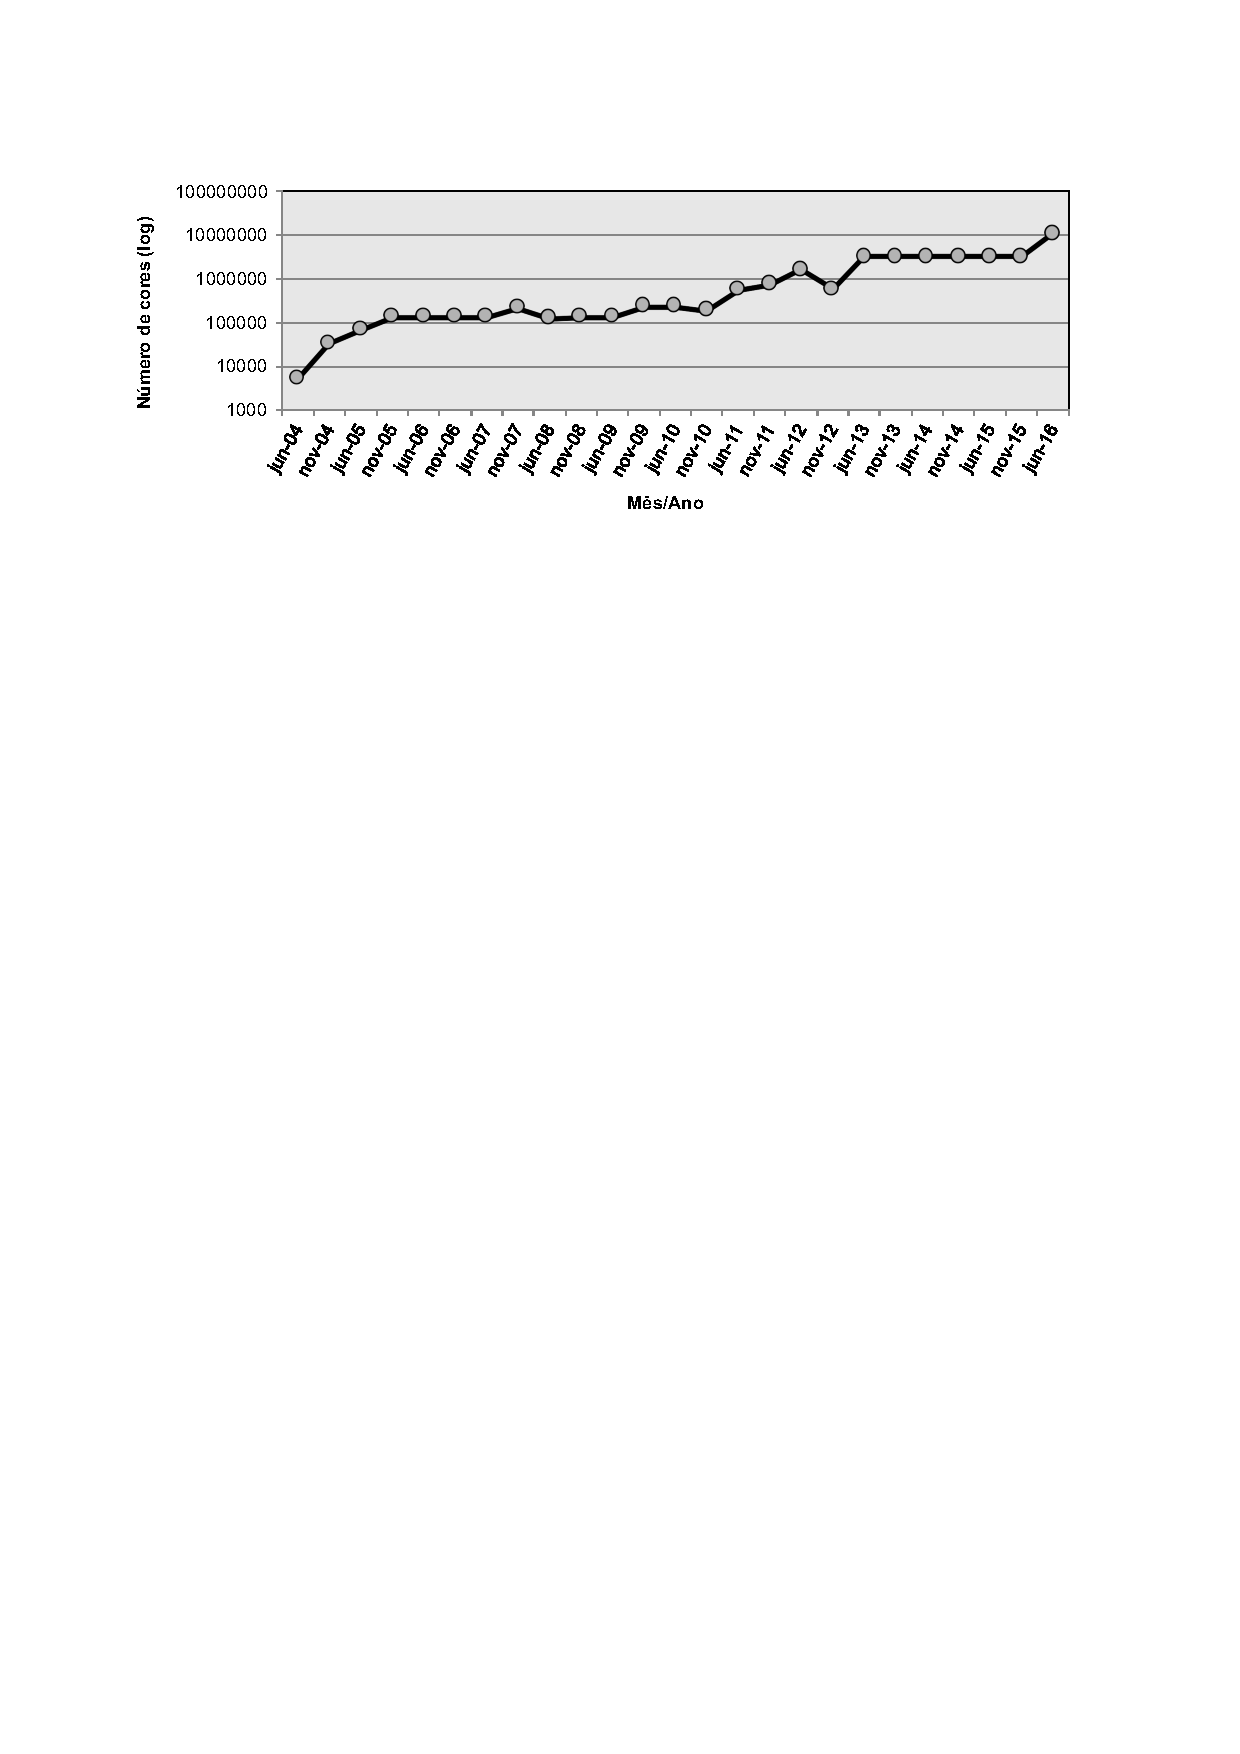
\includegraphics[width=13cm, height=!]{figs/cores-top500.pdf}
		\caption{Número total de núcleos de processamento (\emph{cores}) dos supercomputadores mais poderosos relacionados na lista TOP500.}
		\label{fig:top500}
	\end{figure}

	O desenvolvimento de aplicações paralelas eficientes é um requisito
	obrigatório para que seja possível utilizar todo o potencial dessas.
	Para atingir esse objetivo é necessário o uso de modelos de programação
	paralela. Idealmente, esses modelos devem oferecer um nível de abstração
	alto aos desenvolvedores. Ao mesmo tempo, eles devem fornecer mecanismos
	eficientes para a criação, gerenciamento e orquestração de
	\textit{threads} ou processos.

	Nesse capítulo será apresentado um dos modelos de programação paralela
	muito utilizados na academia e na indústria denominado OpenMP. Esse
	modelo oferece diretivas de compilação que permitem realizar a
	paralelização de trechos de código de maneira transparente. O OpenMP
	oferece uma Interface de Programação de Aplicações (\textit{Application
	Programming Interface} -- API) bastante completa para paralelização de
	aplicações para arquiteturas de memória compartilhada. Nesse tipo de
	arquitetura, diversos processadores ou \textit{cores} tem acesso a uma
	memória principal compartilhada em um único espaço de endereçamento. A
	Figura~\ref{fig:arquitetura-multicore} apresenta uma visão geral de uma
	arquitetura de memória compartilhada.

	\begin{figure}[h]
		\centering
		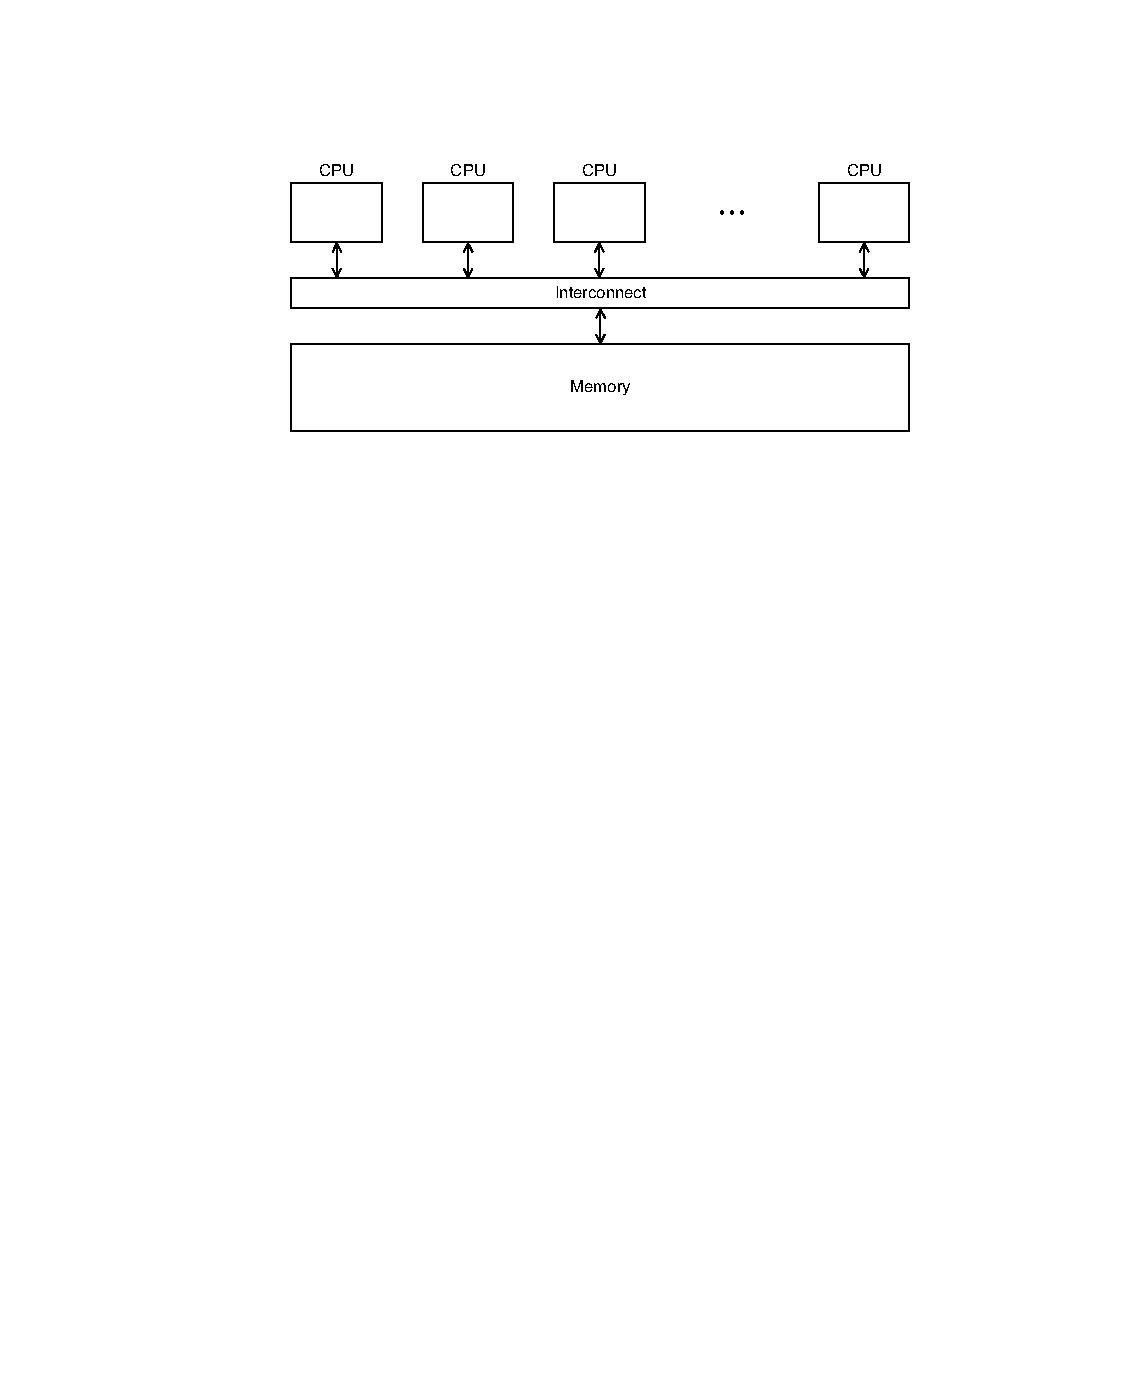
\includegraphics[width=10cm, height=!]{figs/arquitetura-multicore.pdf}
		\caption{Exemplo de uma arquitetura de memória compartilhada.}
		\label{fig:arquitetura-multicore}
	\end{figure}

	Existem duas grandes classes de arquiteturas de memória compartilhada. A
	principal diferença entre elas está relacionado ao tempo de acesso dos
	processadores à memória principal. Em arquiteturas do tipo
	\textit{Uniform Memory Access} (UMA), o tempo de acesso entre o
	processador ou \textit{core} e a memória principal é constante. Por
	outro lado, em arquiteturas do tipo \textit{Non-Uniform Memory Access}
	(NUMA) o tempo de acesso entre o processador ou \textit{core} não é
	constante. A diferença no tempo de acesso vem do fato de que cada
	processador ou \textit{core} tem acesso a bancos de memória local
	(próximos a ele) e também a bancos de memória remotos (distantes a ele
	mas próximos de outro processador ou \textit{core}). Nesse sentido, o
	tempo de acesso à memória principal pode ser pequeno (acesso a um banco
	de memória local) ou grande (acesso a um banco de memória remoto),
	dependendo da distância entre o processador ou \textit{core} e o banco
	de memória que esse processador ou \textit{core} está acessando.
	Arquiteturas utilizadas em \textit{notebooks}, \textit{desktops} ou em
	pequenos servidores que contenham poucas dezenas de \textit{cores} são
	do tipo UMA. Porém, arquiteturas paralelas mais complexas que possuem
	várias dezenas de \textit{cores} são normalmente do tipo NUMA.

\section{Regiões Paralelas e o Modelo Fork-Join}

	Essa seção irá abordar os conceitos básicos de programação paralela com
	OpenMP. Primeiramente, será apresentado o modelo base dessa API, em
	seguida será apresentada a primitiva básica para a criação de regiões
	paralelas no código, e por fim serão apresentadas as formas de
	compartilhamento de dados oferecidas pelo OpenMP.

	% Modelo Fork-Join.
	O OpenMP segue o modelo Fork-Join de execução paralela, que é ilustrado
	na Figura (??). Nesse modelo, o programa inicia sua execução com uma
	única thread, denominada \textit{master thread}. A \textit{master
	thread} executa sequencialmente até encontrar uma região paralela,
	definida pela primitiva \texttt{omp parallel} (Figura (??)). Nesse
	ponto, a \textit{master thread} cria um grupo de threads trabalhadoras,
	denominadas \textit{worker threads} (Figura (??)), e cada \textit{worker
	thread} executa então os comandos delimitados pela região paralela. Ao
	concluirem seu trabalho, as \textit{worker threads} sincronizam suas
	atividades e terminam (Figura (??)). A \textit{master thread} retoma
	então a execução sequencial do programa até que uma nova região paralela
	seja encontrada, momento em que todo esse processo se repete novamente.
	
	% Comentários do Modelo Fork-Join
	Como observação, é importante deixar claro que a \textit{master thread}
	também executa os comandos na região paralela. Assim, se quatro
	\textit{worker threads} são criadas pela \textit{master thread}, um
	total de cinco threads irão executar a região paralela. No entanto, o é
	possível fazer uso de estruturas condicionais alinhadas a funções
	internas do OpenMP para definir uma execução de comandos diferentes para
	a \textit{master thread}. Esse assunto será abordado mais adiante, na
	Seção \ref{section: sincronizacao}. Por fim, vale ressaltar que, em
	implementações modernas do OpenMP, a criação das estruturas internas
	para gerência das threads em regiões paralelas é feita uma única vez,
	quando a primeira região paralela é encontrada. Dessa forma, a
	sobrecarga imposta na aplicação não cresce linearmente com o número de
	regiões paralelas nela presente.

\section{Paralelismo de Dados e Diretivas OpenMP}

	O paralelismo de dados será explorado através do estudo das diretivas de
	compilação disponíveis no OpenMP para paralelização de laços
	(\texttt{omp for} e \texttt{omp parallel for}). Além disso, serão
	discutidas as diferentes estratégias de escalonamento disponíveis no
	ambiente de execução OpenMP (\texttt{static}, \texttt{dynamic} e
	\texttt{guided}) assim como as suas vantages e desvantagens. Por fim,
	será apresentada a cláusula de redução (\texttt{reduction}) juntamente
	com os seus casos de uso.

\section{Paralelismo de Tarefas e Diretivas OpenMP}

	O paralelismo de tarefas será explorado através do estudo das diretivas
	de compilação disponíveis no OpenMP para paralelização de trechos de
	códigos. Serão discutidas duas construções: seções (\texttt{omp
	sections}) e tarefas (\texttt{omp task} e \texttt{omp taskwait}). A
	utilização de tarefas será abordada com o auxilio de problemas
	recursivos clássicos.

\section{Sincronização}
\label{section: sincronizacao}

	Nesse capítulo serão discutidas as diretivas de sincronização de threads
	disponíveis no OpenMP: serialização de código (\texttt{omp single} e
	\texttt{omp master}), exclusão mútua (\texttt{omp critical}) e barreiras
	(\texttt{omp barrier}).

\section{Conclusão}

	Esse capítulo apresentará um apanhado geral do minicurso, ressaltando os
	principais pontos abordados no texto.

\bibliography{referencias}

\end{document}
